\sisetup{
  round-mode = places,
  round-precision = 3,
  exponent-product = \cdot,
  detect-weight=true,
  detect-inline-weight=math,
  tight-spacing = false,
  table-align-text-post = false
}%

\section{Experiments and Results}

To allow for a direct comparison to other state of the art lesion segmentation
methods, we have evaluated our method on the 20 labeled cases from the MICCAI
lesion segmentation challenge \cite{styner20083d}. Data set contains FLAIR, T1,
and T2. In addition, we have added a lesion prior as a forth channel.
\todo{describe what I mean by lesion prior} Our preprocessing pipeline includes
downsampling to \SI{1x1x1}{\milli\metre} resolution, global contrast
normalization, brain extraction. We have then cropped the images to a
\num{159x203x153} region of interest. To evaluate the performance, we have
divided the data set into 5 splits with each split containing 16 images for
training and 4 images for testing such that each image will be used exactly once
for testing. For all experiments, we have used a filter size of \num{9x9x9}, 32
filters and trained the model for 4000 epochs. Training took approximately 36
hours on a single Geforce GTX 760 graphics card. Once the model is trained,
segmentation of a single image can be performed in less than one
second.\todo{Statistics about lesion load (range, mean) for both data sets.}

Figure~\ref{fig:segmentation} shows a comparison of segmentations predicted by
our method with ground truth segmentation for three different cases. The first
two rows illustrate cases were our method performs very well. Our method
achieves a DSC of about 0.61 in both cases, despite the images varying greatly
in contrast, which shows that our method is able to learn features that are
robust to different contrast. The last row illustrates a case were our method
produces more false positives than usually causing a DSC of only 9. This is
caused by the inability of our method to distinguish between diffusely abnormal
white matter and MS lesions. \todo{I would like to say where this issues appear
but I'm also not to sure how to describe the location.} A comparison of our
method with other state of the art methods is summarized in
Table~\ref{tab:state}. Our method outperforms the winning method (Souplet et al.
\cite{souplet2008}) of the MICCAI 2008 challenge and a recently proposed method
based on sparse coding (Weiss et al. \cite{weiss2013}) and performs comparable
with the current state of the art using a combination of carefully designed
features for MS lesion segmentation and random forests (Geremia et al.
\cite{geremia2010}), despite not requiring any domain knowledge.

\begin{figure}[tb]
\centering
\tikz \node[rotate=90,white] {C};
\begin{tabular}{*{6}{p{0.15\textwidth}}}
FLAIR & T1w & T2w & Prior & Ground truth & Our method
\end{tabular}

\tikz \node[rotate=90] {CHB\,07};
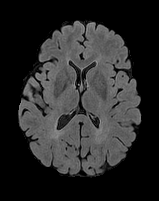
\includegraphics[width=0.15\textwidth]{figures/CHB07-FLAIR-s88}
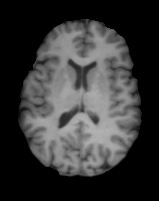
\includegraphics[width=0.15\textwidth]{figures/CHB07-T1w-s88}
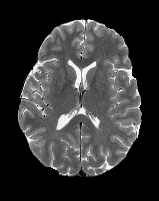
\includegraphics[width=0.15\textwidth]{figures/CHB07-T2w-s88}
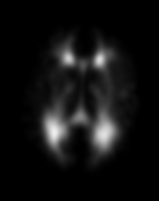
\includegraphics[width=0.15\textwidth]{figures/CHB07-prior-s88}
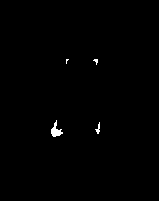
\includegraphics[width=0.15\textwidth]{figures/CHB07-gold-s88}
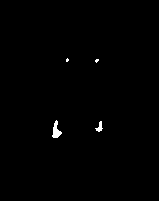
\includegraphics[width=0.15\textwidth]{figures/CHB07-pred-s88} \\
\tikz \node[rotate=90] {CHB\,04};
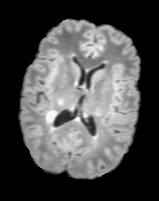
\includegraphics[width=0.15\textwidth]{figures/CHB04-FLAIR-s85}
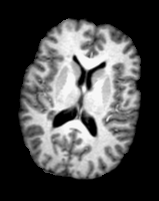
\includegraphics[width=0.15\textwidth]{figures/CHB04-T1w-s85}
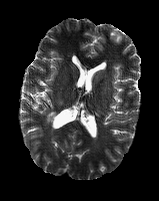
\includegraphics[width=0.15\textwidth]{figures/CHB04-T2w-s85}
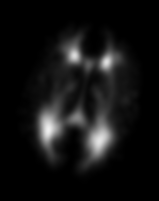
\includegraphics[width=0.15\textwidth]{figures/CHB04-prior-s85}
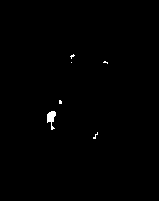
\includegraphics[width=0.15\textwidth]{figures/CHB04-gold-s85}
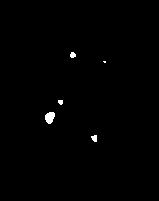
\includegraphics[width=0.15\textwidth]{figures/CHB04-pred-s85} \\
\tikz \node[rotate=90] {UNC\,09};
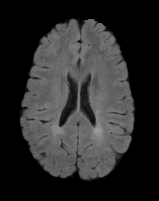
\includegraphics[width=0.15\textwidth]{figures/UNC09-FLAIR-s89}
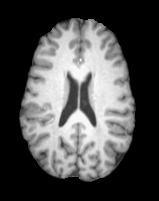
\includegraphics[width=0.15\textwidth]{figures/UNC09-T1w-s89}
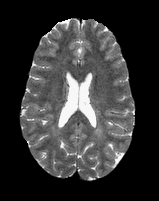
\includegraphics[width=0.15\textwidth]{figures/UNC09-T2w-s89}
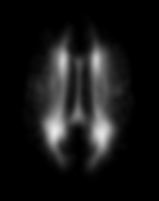
\includegraphics[width=0.15\textwidth]{figures/UNC09-prior-s89}

\includegraphics[width=0.15\textwidth]{figures/UNC09-gold-s89}
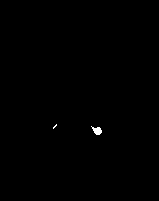
\includegraphics[width=0.15\textwidth]{figures/UNC09-pred-s89}
\caption{Example segmentation using our method. Comment why the method
performed poorly. Maybe it just was a very difficult case. CHB07, FLAIR, T1, T2,
prior, ground truth, predicted segmentation. CHB04, UNC09. Robust to different
contrast, but miss-classifies diffusely abnormal white matter as MS
lesions.}
\label{fig:segmentation}
\end{figure}

\begin{table}[tb]
\def\tabspace{12pt}
\sisetup{
  round-precision = 2,
}%
\caption{Comparison of state of the art methods with our method.}
\label{tab:state}
\centering
\begin{tabular}{l%
@{\hspace{\tabspace}}S[table-format=2.2]
@{\hspace{\tabspace}}S[table-format=2.2]
@{\hspace{\tabspace}}S[table-format=2.2]
}
\toprule
Method & {TPR} & {PPV} & {DSC} \\ 
\midrule
Souplet et al. \cite{souplet2008} & 20.65 & 30.00 & {---} \\ 
Weiss et al. \cite{weiss2013} & 33.00 & 36.85 & 29.05 \\ 
Geremia et al. \cite{geremia2010} & 39.85 & 40.35 & {---}  \\
Our method & 39.71210 & 41.38274 & 35.52401 \\
\bottomrule
\end{tabular}
\end{table}

\begin{table}[tb]
\centering
\sisetup{
round-precision = 1,
}%
\def\Tabspace{7pt}
\def\tabspace{3pt}
\caption{This table is here just for reference. I'm not planning to keep it,
but it shows the full picture of the MICCAI tests.}
\begin{tabular}{l%
% @{\hspace{10pt}}S[table-format=2.1]@{\hspace{\tabspace}}%
% @{\hspace{\tabspace}}S[table-format=2.1]@{\hspace{\Tabspace}}%
% @{\hspace{\Tabspace}}S[table-format=2.1]@{\hspace{\tabspace}}%
% @{\hspace{\tabspace}}S[table-format=2.1]@{\hspace{\Tabspace}}%
% @{\hspace{\Tabspace}}S[table-format=2.1]@{\hspace{\tabspace}}%
% @{\hspace{\tabspace}}S[table-format=2.1]@{\hspace{\tabspace}}%
% @{\hspace{\tabspace}}S[table-format=2.1]@{\hspace{\Tabspace}}%
% @{\hspace{\Tabspace}}S[table-format=2.1]@{\hspace{\tabspace}}%
% @{\hspace{\tabspace}}S[table-format=2.1]@{\hspace{\tabspace}}%
% @{\hspace{\tabspace}}S[table-format=2.1]%
*{10}{S[table-format=2.1]}%
}

\toprule
Patient & \multicolumn{2}{@{\hspace{10pt}}c@{\hspace{10pt}}}{Souplet} &
\multicolumn{2}{c}{Geremia} &
\multicolumn{3}{c}{Weiss} &
\multicolumn{3}{c}{Our method} \\
\addlinespace
 & {TPR} & {PPV} & {TPR} & {PPV} & {TPR} & {PPV} & {DSC} & {TPR} & {PPV} & {DSC}
 \\
\midrule
CHB01 & 22 & 41 & 49 & 64 & 60 & 58 & 59 & 50 & 69 & 58 \\
CHB02 & 18 & 29 & 44 & 63 & 27 & 45 & 34 & 42 & 52 & 46 \\
CHB03 & 17 & 21 & 22 & 57 & 24 & 56 & 34 & 38 & 70 & 49 \\
CHB04 & 12 & 55 & 31 & 78 & 27 & 66 & 38 & 60 & 63 & 61 \\
CHB05 & 22 & 42 & 40 & 52 & 29 & 33 & 31 & 42 & 43 & 42 \\
CHB06 & 13 & 46 & 32 & 52 & 10 & 36 & 16 & 24 & 63 & 35 \\
CHB07 & 13 & 39 & 40 & 54 & 14 & 48 & 22 & 57 & 65 & 61 \\
CHB08 & 13 & 55 & 46 & 65 & 21 & 73 & 32 & 47 & 75 & 58 \\
CHB09 & 3 & 18 & 23 & 28 & 5 & 22 & 8 & 22 & 49 & 30 \\
CHB10 & 5 & 18 & 23 & 39 & 15 & 12 & 13 & 11 & 64 & 19 \\
\addlinespace
UNC01 & 1 & 1 & 2 & 1 & 33 & 29 & 31 & 3 & 6 & 4 \\
UNC02 & 37 & 39 & 48 & 36 & 54 & 51 & 53 & 54 & 38 & 44 \\
UNC03 & 12 & 16 & 24 & 35 & 64 & 27 & 38 & 62 & 28 & 39 \\
UNC04 & 38 & 54 & 54 & 38 & 40 & 51 & 45 & 59 & 35 & 44 \\
UNC05 & 38 & 8 & 56 & 19 & 25 & 10 & 16 & 10 & 5 & 6 \\
UNC06 & 57 & 9 & 15 & 8 & 13 & 55 & 20 & 24 & 49 & 32 \\
UNC07 & 27 & 18 & 76 & 16 & 44 & 23 & 30 & 33 & 19 & 24 \\
UNC08 & 27 & 20 & 52 & 32 & 43 & 13 & 20 & 51 & 13 & 20 \\
UNC09 & 16 & 43 & 67 & 36 & 69 & 6 & 11 & 51 & 5 & 9 \\
UNC10 & 22 & 28 & 53 & 34 & 43 & 23 & 30 & 56 & 19 & 28 \\
\addlinespace
Average & 20.65 & 30.00 & 39.85 & 40.35 & 33.00 & 36.85 & 29.05 & 39.71 & 41.38
& 35.52
\\
\bottomrule
\end{tabular}
\end{table}

\begin{table}[tb]
\sisetup{
  round-precision = 2,
}% 
\centering
\caption{Comparison of segmentation performance on the training and test set
for varying number of training samples. The difference between training and
test performance is reduces for increasing number of training samples. A
training set size of 150 is sufficient to prevent overfitting.}
\label{tab:bioms}
\begin{tabular} {c*{6}{S[table-format=3.3]}}
\toprule
Number of & \multicolumn{3}{c}{Training set} &
\multicolumn{3}{c}{Test set}
\\
training samples & {TPR} & {PPV} & {DSC} & {TPR} & {PPV} & {DSC} \\
\midrule 
5 & 77.9679 & 66.2261 & 70.9317 & 47.1575 & 57.0428 & 48.5493 \\
10 & 73.4045 & 68.1603 & 69.7124 & 55.0416 & 59.8499 & 53.9332 \\
15 & 71.765 & 68.234 & 68.8614 & 56.2786 & 60.883 & 55.4736 \\
25 & 69.3865 & 70.6347 & 68.9442 & 57.4285 & 61.0626 & 56.2912 \\
250 & 64.5539 & 58.2538 & 58.5023 & 65.4692 & 56.813 & 57.5434 \\
\bottomrule
\end{tabular}
\end{table}

To evaluate the impact of the training set size on the segmentation performance,
we have evaluated our model on different subsets of a data set from an MS clinical
trail. With data set contained T2w and PDw images from 500 subjects at a single
time point. We have divided the data set into a training and test set containing
250 images each. We have then trained our model on a varying number of image
from the training set and evaluated the segmentation performance on the
selected training samples and all images of the test set. The result of this
test is illustrated in Table~\ref{tab:bioms}. For very small number of training
samples, our model achieves a DSC of 71 in the training set and 49 in the test
set. The large difference between the results on the training and test set
indicates that the training sample size is not sufficient to prevent
overfitting. As we increase the number of training samples, the difference
between the results on the training and test set decreases. At 150 samples, the
performance on the training set is almost as good as on the test set, which
indicates that our model is not overfitting. We also do not see an improvement
thereafter. For this study, if have trained a relatively simple model with only
2 layers and 32 filters per layer. We expect that models with more layers and
filters are more prone to overfitting for smaller training set sizes, but might
keep improving beyond 150 samples.



% \paragraph{Training Pipeline}
% \begin{itemize}
% \item Downsample training images and training segmentations from
% \SI{0.5x0.5x0.5}{\milli\meter} to \SI{1x1x1}{\milli\meter} voxel resolution.
% \item Perform brain extraction
% \item Crop to smallest ROI
% \item Pad all images to standard size
% \item[$\Rightarrow$] Calculate combined cropping parameters
% \item Perform training of the NN on the downsampled training set
% \item Calculate probability maps for the entire downsampled training set
% \item Upsample the probability maps to the native resolution
% \item Crop lesion masks in native resolution to fit the same ROI as the
% upsampled probability masks
% \item Choose the threshold that maximizes the DSC in the training set 
% \end{itemize}

% \paragraph{Experiments to come}
% 
% \begin{itemize}
% 
% \item \emph{Optional}\quad Evaluation on BioMS using stride-1 convolutions and
% new pre-processing pipeline with and without lesion prior, with individual and
% shared bias terms. Metrics: TPR, PPV, DSC, correlations with lesion load and
% clinical scores.
% 
% \end{itemize}


% \begin{table}
% \caption{Segmentation results measured using the Dice Similarity Coefficient.
% Two layer auto-encoder, stride size of \num{2x2x1}, 32 filters, sensitivity
% ratio 0.05. Threshold finding methods: a) using a global threshold that
% optimizes the average DSC of the entire data set, b) using the optimal
% thresholds for each sample, and c) using predicted thresholds for each sample.}
% \label{tab:segmentation}
% \centering
% \def\tabspace{10pt}
% \sisetup{
%   round-precision = 3,
% }%
% % \small
% \begin{tabular}{@{}l%
% @{\hspace{\tabspace}}S[table-format=1.3]%
% @{\hspace{\tabspace}}S[table-format=1.3]
% @{\hspace{\tabspace}}S[table-format=1.3]
% @{\hspace{\tabspace}}S[table-format=1.3]
% @{\hspace{\tabspace}}S[table-format=1.3]
% @{\hspace{\tabspace}}S[table-format=1.3]
% @{}}
% \toprule
% Method & \multicolumn{6}{c}{DSC per Lesion Load Category} \\
% \addlinespace
%  & {0.0--4.0} & {4.0--7.8} & {7.8--14.7} & {14.7--28.5} & {$>28.5$} &
% {Average} \\
% \midrule
% Global threshold &  0.297805 & 0.545574 & 0.60051 & 0.650483 & 0.679614 &
%  0.543181 \\
% Optimal thresholds & 0.351185 & 0.568412 & 0.618115 & 0.667473 & 0.727397 &
% 0.572716 \\
% Predicted thresholds & 0.337834 & 0.550028 & 0.587458 & 0.653475 &
% 0.716976 & 0.555662 \\
% \bottomrule
% \end{tabular}
% \end{table}
% 
% \begin{table}
% \caption{Correlations with biomarkers is comparable to the expert
% segmentations. Threshold methods are: global threshold (LLG), optimal threshold
% (LLO), and predicted threshold (LLP).}
% \label{tab:cross}
% \centering
% \def\tabspace{14pt}
% \begin{tabular}{c%
% @{\hspace{\tabspace}}S[table-format=1.4]%
% @{\hspace{\tabspace}}S[table-format=2.6]%
% @{\hspace{\tabspace}}S[table-format=2.6]%
% @{\hspace{\tabspace}}S[table-format=2.6]%
% @{\hspace{\tabspace}}S[table-format=1.5]%
% @{\hspace{\tabspace}}S[table-format=1.6]%
% }
% \toprule
%      & {T25W} & {9-HPT} & {PASAT} & {MSFC} & {EDSS} & {T2LL} \\
% \midrule
% LLG & 0.0889204058874592 & -0.299046682079096*** & -0.35652944988915*** & -0.414587036427664*** & 0.111910491023784* & 0.867904019287295*** \\
% LLO & 0.0955077933828887* & -0.29002627967845*** & -0.36828512897955*** & -0.41898534832637*** & 0.116889743878327* & 0.988979555746338*** \\
% LLP & 0.0896915607291051 & -0.300773510817976*** & -0.342386015914701*** & -0.411524441008343*** & 0.134054634214833** & 0.869216107742852*** \\
% \addlinespace
% T2LL & 0.0830609699877066 & -0.288809520550953*** & -0.370891003440786*** &
% -0.415459123322053*** & 0.121219714387235* & {---} \\
% \bottomrule
% \end{tabular}
% \end{table}

